% Template file for a standard thesis
\documentclass[11pt]{isuthesis}
\usepackage[pdftex]{graphicx}

% Standard, old-style thesis
%\usepackage{isutraditional}   \chaptertitle

% Old-style, thesis numbering down to subsubsection
\alternate
\usepackage{rotating}
% Bibliography without numbers or labels
\usepackage{natbib}
\bibliographystyle{apa}
%\includeonly{titletoc,chapter1}
%Optional Package to add PDF bookmarks and hypertext links
\usepackage[pdftex,hypertexnames=false,linktocpage=true]{hyperref}
\hypersetup{colorlinks=true,linkcolor=blue,anchorcolor=blue,citecolor=blue,filecolor=blue,urlcolor=blue,bookmarksnumbered=true,pdfview=FitB}

% Note sure why this is necessary
% http://tex.stackexchange.com/questions/257418/error-tightlist-converting-md-file-into-pdf-using-pandoc
\providecommand{\tightlist}{%
  \setlength{\itemsep}{0pt}\setlength{\parskip}{0pt}}


\begin{document}

% Template Titlepage File
\title{This is the title of a thesis
submitted to Iowa State University\\
Note that only the first letter of
the first word and proper names
are capitalized}
\author{Wilbur Terrance Johnson}
\degree{MASTER OF SCIENCE}
\major{Human Development and Family Studies (Marriage and Family Therapy)}
\level{master's}
\mprof{Susan D. Ross}
\members{Mary Jones \\ Bjork Petersen}
\notice
% Add these additional lines for a Doctoral Dissertation
%\degree{DOCTOR OF PHILOSOPHY}
%\level{doctoral}
%\format{dissertation}
%\committee{4}
%\members{Mary Jones \\ Bjork Petersen \\ Sam Anders \\ Harold Jones}
% Add these additional lines for a Creative Component
% - also comment out the \maketitle command
%\format{Creative Component}
%\submit{the graduate faculty}
\maketitle


% Table of Contents, List of Tables and List of Figures
\pdfbookmark[1]{TABLE OF CONTENTS}{table}
\tableofcontents
\addtocontents{toc}{\def\protect\@chapapp{}} \cleardoublepage \phantomsection
\addcontentsline{toc}{chapter}{LIST OF TABLES}
\listoftables
\cleardoublepage \phantomsection \addcontentsline{toc}{chapter}{LIST OF FIGURES}
\listoffigures
% Comment out the next line if NOT using chaptertitle
% \addtocontents{toc}{\def\protect\@chapapp{CHAPTER\ }}

\specialchapt{ABSTRACT}

The following describes a collection of software interfaces for data acquisiton and visualization. All of these interfaces are freely available as extension packages to the R language and leverage web technologies to achieve accessible, portable, and reproducible workflows. The majority of this work (LDAvis, animint, and plotly) focuses on interactive visualization. These interfaces fall roughly into two categories: (1) domain-specific (LDAvis) and (2) general purpose tools for interactive data visualization (animint and plotly). More specifially, the LDAvis package produces an interactive visualization to aid interpretation of Latent Dirichlet Allocation (LDA) model output. The animint and plotly packages are more general, and build upon principles from the grammar of graphics, but extend those principles in slightly different ways to enable interactivity, such as animation and brushing a scatterplot matrix. 

\chapter{Literature Review}\label{literature-review}

\section{What makes a good software
interface?}\label{what-makes-a-good-software-interface}

Unwin and Hofmann \citep{Unwin:1999vp} discuss the strengths,
weaknesses, and differences between using graphical and command-line
interfaces for data analysis. Graphical user interfaces (GUIs) can be
much more intuitive to use, but at the cost of being less flexible,
precise, and repeatable. Unwin and Hofmann argue statistical software
should strive to achieve a synergy of two that leverages both of their
strengths. That is, a command-line interface when we can precisely
describe what we want and a graphical interface for ``searching for
information and interesting structures without fully specified
questions.''

Unwin and Hofmann further discuss the different audiences these
interfaces attract. Command-line interfaces typically attract ``power
users'' such as applied statisticians and statistical researchers in a
university, whereas more casual users of statistical software typically
prefer a GUI. In later sections, we discuss GUIs in greater detail
within the context of interactive statistical graphics. For now, we
briefly discuss some best practices for designing a command-line
interface for statistical computing in R.

Before authoring an interface, one should establish the target audience,
the class of problems it should address, and loosely define how the
interface should actually work. During this process, it may also be
helpful to identify your audience as being primarily composed of
\emph{software developers} or \emph{data analysts}. Developers are
typically more interested in using the interface to develop novel
software or incorporating the functionality into a larger scientific
computing environment \citep{embedded-computing}. In this case,
interactive exploration and troubleshooting is not always a luxury, so
robust functionality is of utmost importance. On the other hand,
analysts interfaces should work well in an interactive environment since
this caters to rapid prototyping of ideas and troubleshooting of errors.

Good developer interfaces often make it easier to implement good analyst
interfaces. A great recent example of a good developer interface is the
R package \textbf{Rcpp}, which provides a seamless interface between R
with C++ \citep{Rcpp}. To date, more than 500 R packages use
\textbf{Rcpp} to make interfaces that are both expressive and efficient,
including the highly influential analyst interfaces such as
\textbf{tidyr} and \textbf{dplyr} \citep{tidy-data}; \citep{dplyr}.
These interfaces help analysts focus on the primary task of wrangling
data into a form suitable for visualization and statistical modeling,
rather than focusing on the implementation details behind how the
transformations are performed. \citep{Donoho:2015tu} argues that these
interfaces ``May have more impact on today's practice of data analysis
than many highly-regarded theoretical statistics papers''.

Evaluating statistical computing interfaces is certainly a subjective
matter since we all have different tastes, different backgrounds, and
have different needs. It seems reasonable to evaluate an interface based
on its effectiveness and efficiency in aiding a user complete their
task, but as \citep{Unwin:1999vp} points out, ``There is a tendency to
judge software by the most powerful tools they provide (whether with a
good interface or not)''. As a result, all too often, analysts must
spend time gaining the skills of a software developer. Good analyst
interfaces often abstract functionality from developer interfaces in a
way that allow analysts to focus on their primary task of
acquiring/analyzing/modeling/visualizing data, rather than the
implementation details. The following focuses on such work with respect
to acquiring data from the web and interactive statistical web graphics.

\section{Acquiring and wrangling web content in
R}\label{acquiring-and-wrangling-web-content-in-r}

\subsection{Interfaces for working with web
content}\label{interfaces-for-working-with-web-content}

R has a rich history of interfacing with web technologies for
accomplishing a variety of tasks such as requesting, manipulating, and
creating web content. As an important first step, extending ideas from
\citep{Chambers:1999}, Brian Ripley implemented the connections
interface for file-oriented input/output in R \citep{Connections}. This
interface supports a variety of common transfer protocols (HTTP, HTTPS,
FTP), providing access to most files on the web that can be identified
with a Uniform Resource Locator (URL). Connection objects are actually
external pointers, meaning that, instead of immediately reading the
file, they just point to the file, and make no assumptions about the
actual contents of the file.

Many functions in the base R distribution for reading data (e.g.,
\texttt{scan}, \texttt{read.table}, \texttt{read.csv}, etc.) are built
on top of connections, and provide additional functionality for parsing
well-structured plain-text into basic R data structures (vector, list,
data frame, etc.). However, the base R distribution does not provide
functionality for parsing common file formats found on the web (e.g.,
HTML, XML, JSON). In addition, the standard R connection interface
provides no support for communicating with web servers beyond a simple
HTTP GET request \citep{Lang:2006us}.

The \textbf{RCurl}, \textbf{XML}, and \textbf{RJSONIO} packages were
major contributions that drastically improved our ability to request,
manipulate, and create web content from R \citep{nolan-lang}. The
\textbf{RCurl} package provides a suite of high and low level bindings
to the C library libcurl, making it possible to transfer files over more
network protocols, communicate with web servers (e.g., submit forms,
upload files, etc.), process their responses, and handle other details
such as redirects and authentication \citep{RCurl}. The \textbf{XML}
package provides low-level bindings to the C library libxml2, making it
possible to download, parse, manipulate, and create XML (and HTML)
\citep{XML}. To make this possible, \textbf{XML} also provides some data
structures for representing XML in R. The \textbf{RJSONIO} package
provides a mapping between R objects and JavaScript Object Notation
(JSON) \citep{RJSONIO}. These packages were heavily used for years, but
several newer interfaces have made these tasks easier and more
efficient.

The \textbf{curl}, \textbf{httr}, and \textbf{jsonlite} packages are
more modern R interfaces for requesting content on the web and
interacting with web servers. The \textbf{curl} package provides a much
simpler interface to libcurl that also supports streaming data (useful
for transferring large data), and generally has better performance than
\textbf{RCurl} \citep{curl}. The \textbf{httr} package builds on
\textbf{curl} and organizes it's functionality around HTTP verbs (GET,
POST, etc.) \citep{httr}. Since most web application programming
interfaces (APIs) organize their functionality around these same verbs,
it is often very easy to write R bindings to web services with
\textbf{httr}. The \textbf{httr} package also builds on
\textbf{jsonlite} since it provides consistent mappings between R/JSON
and most most modern web APIs accept and send messages in JSON format
\citep{jsonlite}. These packages have already had a profound impact on
the investment required to interface R with web services, which are
useful for many things beyond data acquisition. For example, it is now
easy to install R packages hosted on the web (\textbf{devtools}),
perform cloud computing (\textbf{analogsea}), and archive/share
computational outputs (\textbf{dvn}, \textbf{rfigshare},
\textbf{RAmazonS3}, \textbf{googlesheets}, \textbf{rdrop2}, etc.).

The \textbf{rvest} package builds on \textbf{httr} and makes it easy to
manipulate content in HTML/XML files \citep{rvest}. Using \textbf{rvest}
in combination with \href{http://selectorgadget.com/}{SelectorGadget},
it is often possible to extract structured information (e.g., tables,
lists, links, etc) from HTML with almost no knowledge/familiarity with
web technologies. The \textbf{XML2R} package has a similar goal of
providing an interface to acquire and manipulate XML content into
tabular R data structures without any working knowledge of
XML/XSLT/XPath \citep{Sievert:2014a}. As a result, these interfaces
reduce the startup costs required for analysts to acquire data from the
web.

Packages such as \textbf{XML}, \textbf{XML2R}, and \textbf{rvest} can
download and parse the source of web pages, which is \emph{static}, but
extracting \emph{dynamic} web content requires additional tools. The R
package \textbf{rdom} fills this void and makes it easy to render and
access the Document Object Model (DOM) using the headless browsing
engine phantomjs \citep{rdom}. The R package \textbf{RSelenium} can also
render dynamic web pages and simulate user actions, but its broad scope
and heavy software requirements make it harder to use and less reliable
compared to \textbf{rdom} \citep{RSelenium}. \textbf{rdom} is also
designed to work seamlessly with \textbf{rvest}, so that one may use the
\texttt{rdom()} function instead of \texttt{read\_html()} to render,
parse, and return the DOM as HTML (instead of just the HTML page
source).

Any combination of these R packages may be useful in acquiring data for
personal use and/or providing a higher-level interface to specific data
source(s) to increase their accessibility. The next section focuses on
such interfaces.

\subsection{Interfaces for acquiring data on the
web}\label{interfaces-for-acquiring-data-on-the-web}

The web provides access to the world's largest repository of publicly
available information and data. This provides a nice \emph{potential}
resource both teaching and practicing applied statistics, but to be
practical useful, it often requires a custom interface to make data more
accessible. If publishers follow best practices, a custom interface to
the data source usually is not needed, but this is rarely the case. Many
times structured data is embedded within larger unstructured documents,
making it difficult to incorporate into a data analysis workflow. This
is especially true of data used to inform downstream web applications,
typically in XML and/or JSON format. There are two main ways to make
such data more accessible: (1) package, document, and distribute the
data itself (2) provide functionality to acquire the data.

If the data source is fairly small, somewhat static, and freely
available with an open license, then we can directly provide data via R
packaging mechanism. In this case, it is best practice for package
authors include scripts used to acquire, transform, and clean the data.
This model is especially nice for both teaching and providing examples,
since users can easily access data by installing the R package.
\citep{rpkgs} provides a nice section outlining the details of bundling
data with R packages.\footnote{This section is freely available online
  \url{http://r-pkgs.had.co.nz/data.html}.}

R packages that just provide functionality to acquire data can be more
desirable than bundling it for several reasons. In some cases, it helps
avoid legal issues with rehosting copyrighted data. Furthermore, the
source code of R packages can always be inspected, so users can verify
the cleaning and transformations performed on the data to ensure its
integrity, and suggest changes if necessary. They are also versioned,
which makes the data acquisition, and thus any downstream analysis, more
reproducible and transparent. It is also possible to handle dynamic data
with such interfaces, meaning that new data can be acquired without any
change to the underlying source code. As explained in
\protect\hyperlink{taming-pitchfx-data-with-xml2r-and-pitchrx}{Taming
PITCHf/x Data with XML2R and pitchRx}, this is an important quality of
the \textbf{pitchRx} R package since new PITCHf/x data is made available
on a daily basis.

Perhaps the largest centralized effort in this domain is lead by
\href{https://ropensci.org}{rOpenSci}, a community of R developers that,
at the time of writing, maintains more than 50 packages providing access
to scientific data ranging from bird sightings, species occurrence, and
even text/metadata from academic publications. This provides a
tremendous service to researchers who want to spend their time building
models and deriving insights from data, rather than learning the
programming skills necessary to acquire and clean it.

It's becoming increasingly clear that ``meta'' packages that standardize
the interface to data acquisition/curation in a particular domain would
be tremendously useful. However, it is not clear how such interfaces
should be designed. The R package \textbf{etl} is one step in this
direction and aims to provide a standardized interface for \emph{any}
data access package that fits into an Extract-Transform-Load paradigm
\citep{etl}. The package provides generic
\texttt{extract}-\texttt{transform}-\texttt{load} functions, but
requires package authors to write custom
\texttt{extract}-\texttt{transform} methods for the specific data
source. In theory, the default \texttt{load} method works for any
application; as well as other database management operations such as
\texttt{update} and \texttt{clean}.

\section{Dynamic interactive statistical web
graphics}\label{dynamic-interactive-statistical-web-graphics}

\subsection{Why interactive?}\label{why-interactive}

Unlike computer graphics which focuses on representing reality,
virtually; data visualization is about garnering abstract relationships
between multiple variables from visual representation. The
dimensionality of data, the number of variables can be anything, usually
more than 3D, which summons a need to get beyond 2D canvasses for
display. Technology enables this, enabling the user to see many views,
query and link components. As demonstrated in Figure \ref{fig:tour}
using the R package \textbf{tourbrush} \citep{tourbrush}, interactive
and dynamic graphics allow us to go beyond the constraints of
low-dimensional displays to see high-dimensional relationships in data.

\begin{figure}

{\centering 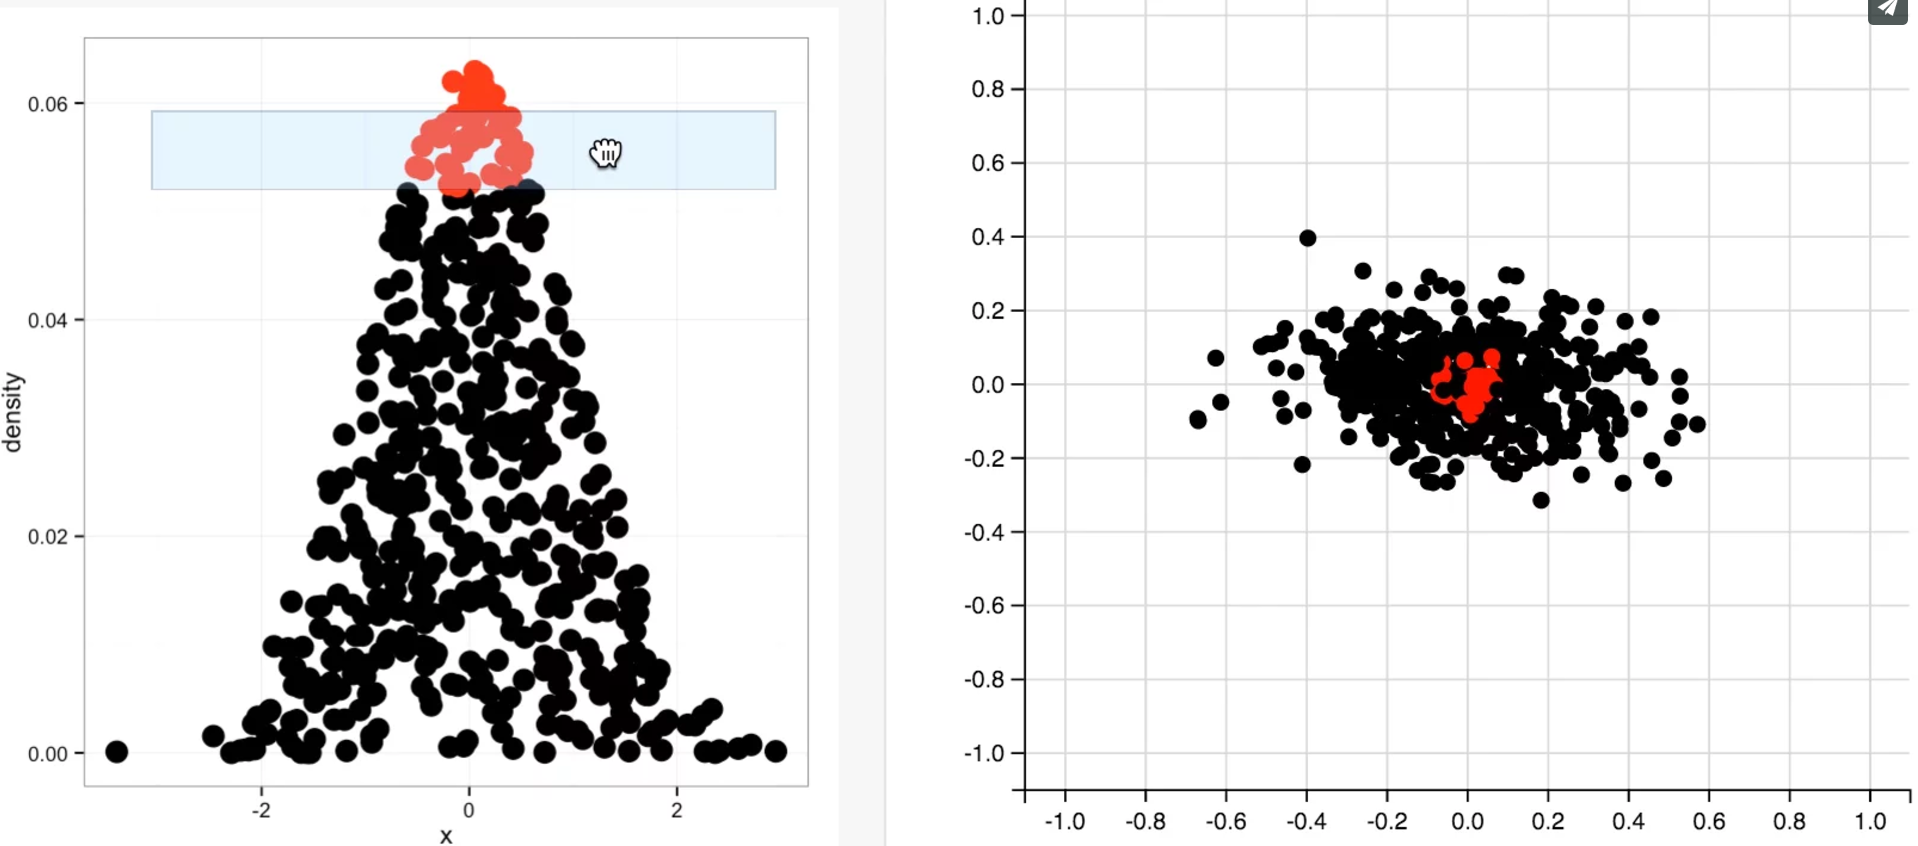
\includegraphics[width=26.64in]{diagrams/tourbrush} 

}

\caption{A demonstration of interactive and dynamic techniques for visualizing high-dimensional relationships in data using the R package **tourbrush**. You can view this movie online at https://vimeo.com/148050343 or via the supplementary materials}\label{fig:tour}
\end{figure}

Dynamic interactive statistical graphics is useful for descriptive
statistics, and also to help build better inferential models. Any
statistician is familiar with diagnosing a model by plotting data in the
model space (e.g., residual plot, qqplot). This works well for
determining if the assumptions of a model are adequate, but rarely
suggests that our model neglects important features in the data. To
combat this problem, \citep{Wickham:2015ur} suggest that we should plot
the model in the data space and use dynamic interactive statistical
graphics to do so. Interactive graphics have also proved to be useful
for exploratory model analysis, a situation where we have many models to
evaluate, compare, and critique \citep{Unwin:2003uy};
\citep{Urbanek:2004}; \citep{Ripley:2004}; \citep{Unwin:2006};
\citep{Wickham:2007wq}. With such power comes responsibility that we can
verify that visual discoveries are real, and not due to random chance
\citep{Buja:2009hp}; \citep{Majumder:2013ie}.

The ASA Section on Statistical Computing and Graphics maintains a video
library which captures many useful dynamic interactive statistical
graphics techniques. Several videos show how xgobi (predecessor to
ggobi), a dynamic interactive statistical graphics system, can be used
to reveal high-dimensional relationships and structures that cannot be
easily identified using numerical methods alone \citep{xgobi}.\footnote{For
  example, \url{http://stat-graphics.org/movies/xgobi.html} and
  \url{http://stat-graphics.org/movies/grand-tour.html}} Another notable
video shows how the interactive graphics system mondrian can be used to
quickly find interesting patterns in high-dimensional data using
exploratory data analysis (EDA) techniques
\citep{mondrianbook}.\footnote{\url{http://stat-graphics.org/movies/tour-de-france.html}}
The most recent video shows how dynamic interactive techniques can help
interpret a topic model (a statistical mixture model applied to text
data) using the R package \textbf{LDAvis} \citep{Sievert:2014b}, which
is the first web-based visualization in the library, and is discussed at
depth in
\protect\hyperlink{ldavis-a-method-for-visualizing-and-interpreting-topics}{LDAvis:
A method for visualizing and interpreting topics}.

In order to be practically useful, interactive statistical graphics must
be fast, flexible, accessible, portable, and reproducible. In general,
over the last 20-30 years interactive graphics systems were fast and
flexible, but were generally not easily accessible, portable, or
reproducible. The web browser provides a convenient platform to combat
these problems. For example, any visualization created with
\textbf{LDAvis} can be shared through a Uniform Resource Locator (URL),
meaning that anyone with a web browser and an internet connection can
view and interact with a visualization. Furthermore, we can link anyone
to any possible state of the visualization by encoding selections with a
URL fragment identifier. This makes it possible to link readers to an
interesting state of a visualization from an external document, while
still allowing them to independently explore the same visualization and
assess conclusions drawn from it.\footnote{A good example of is
  \url{http://cpsievert.github.io/LDAvis/reviews/reviews.html}}

\subsection{Indirect versus direct
manipulation}\label{indirect-versus-direct-manipulation}

Even within the statistical graphics community, the term
\emph{interactive} graphics can mean wildly different things to
different people \citep{swayne-klinke}. Some early statistical
literature on the topic uses interactive in the sense that an
interactive command-line prompt allows users to create graphics
on-the-fly \citep{S:1984}. That is, users enter commands into the
command-line prompt, the prompts evaluates the command, and prints the
result (known as the read--eval--print loop (REPL)). Modifying a command
to generate another variation of a particular result (e.g., to restyle a
static plot) can be thought of as a type of interaction that some might
call \emph{indirect manipulation}.

Indirect manipulation can be achieved both from the command-line or from
a graphical user interface (GUI). Indirect manipulation from the
command-line is more flexible since we have complete control over the
commands, but it is also more cumbersome since we must translate our
thoughts into code. Indirect manipulation via a GUI is more restrictive,
but it helps reduces the gulf of execution (i.e., easier to generate
desired output) for end-users \citep{Hutchins:1985wu}. In this sense, a
GUI can be useful, even for experienced programmers, when the
command-line interface impedes our primary task of deriving insight from
data.

In many cases, the gulf of execution can be further reduced through
direct manipulation. Roughly speaking, within the context of interactive
graphics, direct manipulation occurs whenever we interact with a plot
and reveal new information tied to the event. \citet{ggobi:2007} use the
terms dynamic graphics and direct manipulation to characterize ``plots
that respond in real time to an analyst's queries and change dynamically
to re-focus, link to information from other sources, and re-organize
information.'' Perhaps the most powerful direct manipulation technique
is the paradigm of linked views \citep{Wilhelm:2005}, which will be
discussed in more detail in a later section.

A simple example to help demonstrate the differences between these
interactive techniques would be in an analysis of variance (ANOVA) via
multiple boxplots. By default, most plotting libraries sort categories
alphabetically, but this is usually not optimal for visual comparison of
groups. With a static plotting library such as \textbf{ggplot2}, we
could indirectly manipulate the default by going back to the
command-line, reordering the factor levels of the categorical variables,
and regenerate the plot \citep{ggplot2}. This is flexible and precise
since we may order the levels by any measure we wish (e.g., Median,
Mean, IQR, etc.), but it would be much quicker and easier if we had a
GUI with a drop-down menu for most of the reasonable sorting options. In
a general purpose interactive graphics system such as mondrian, one can
use direct manipulation to directly click and drag on the categories to
reorder them, making it quick and easy to compare any two groups of
interest \citep{mondrianbook}.

\subsection{Linked views and
pipelines}\label{linked-views-and-pipelines}

A general purpose interactive statistical graphics system should possess
many direct manipulation techniques such as identifying (i.e., mousing
over points to reveal labels), focusing (i.e., view size adjustment, pan
and zoom), brushing/identifying, etc. However, it is the intricate
management of information across multiple views of data in response to
user events that is most valuable. Extending ideas from
\citep{viewing-pipeline}, \citep{plumbing} point out that any
visualization system with linked views must implement a data pipeline.
That is, a ``central commander'' must be able to handle interaction(s)
with a given view, translate its meaning to the data space, and update
any linked view(s) accordingly. In order to do so, the commander must
know, and be able to compute, function(s) from data to visual space, as
well as from visual space to the data. Implementing a pipeline that is
fast, general, and able to handle statistical transformations is
incredibly difficult. Unfortunately, literature on the implementation of
such pipelines is virtually non-existent, but \citet{Xie:2014co}
provides a nice overview of the implementation details in the R package
\textbf{cranvas} \citep{cranvas}.

\subsection{Web graphics}\label{web-graphics}

Thanks to the constant evolution and eventual adoption of HTML5 as a web
standard, the modern web browser now provides a viable platform for
building an interactive statistical graphics systems. HTML5 refers to a
collection of technologies, each designed to perform a certain task,
that work together in order to present content in a web browser. The
Document Object Model (DOM) is a convention for managing all of these
technologies to enable \emph{dynamic} and \emph{interactive} web pages.
Among these technologies, there are several that are especially relevant
for interactive web graphics:

\begin{enumerate}
\def\labelenumi{\arabic{enumi}.}
\tightlist
\item
  HTML: A markup language for structuring and presenting web content.
\item
  SVG: A markup language for drawing scalable vector graphics.
\item
  CSS: A language for specifying styling of web content.
\item
  JavaScript: A language for manipulating web content.
\end{enumerate}

Juggling all of these technologies just to create a simple statistical
plot is a tall order. Thankfully, HTML5 technologies are publicly
available, and benefit from thriving community of open source developers
and volunteers. In the context of web-based visualization, the most
influential contribution is Data Driven Documents (D3), a JavaScript
library which provides high-level semantics for binding data to web
content (e.g., SVG elements) and orchestrating scene updates/transitions
\citep{Bostock:2011}. D3 is wildly successful because is builds upon web
standards, without abstracting them away, which fosters customization
and interoperability. However, compared to a statistical graphics
environments like R, creating basic charts is complicated, and a large
amount of code must be hard-wired to each visualization. Fortunately,
there are a number of ways to provide higher-level interfaces to web
graphics, and we focus on R interfaces.

\subsection{Translating R graphics to the
web}\label{translating-r-graphics-to-the-web}

There are a few ways to simply translate R graphics to a web format,
such as SVG. R has built-in support for a SVG graphics device, made
available through the \texttt{svg()} function, but it can be quite slow,
which inspired the new \textbf{svglite} package \citep{svglite}. The
\textbf{SVGAnnotation} package provides some functionality to
post-process SVG files generated with \texttt{svg()} to add some basic
interactivity and animation \citep{SVGAnnotation}. The \textbf{gridSVG}
package is specially designed to translate \textbf{grid} graphics (e.g.,
\textbf{ggplot2}, \textbf{lattice}, etc.) to SVG, and preserves the
naming information of grid objects, making it easier to layer on
interactive functionality \citep{gridSVGreport}. \citet{vdmR} uses
\textbf{gridSVG} to enable linked brushing between \textbf{ggplot2}
graphics, but only implements a few chart types. \citet{svgPanZoom} uses
\textbf{gridSVG} to provide pan and zoom capability to virtually any R
graphic.

The \textbf{animint} and \textbf{plotly} packages take a different
approach to translating \textbf{ggplot2} graphics to a web format
\citep{animint}; \citep{plotly}. Instead of translating directly to SVG
via \textbf{gridSVG}, they extract relevant information from the
internal representation of a \textbf{ggplot2} graphic\footnote{For a
  visual display of the internal representation used to render a
  \textbf{ggplot2} graph, see my \textbf{shiny} app here
  \url{https://gallery.shinyapps.io/ggtree}.}, store it in JavaScript
Object Notation (JSON), and pass the JSON as input to a JavaScript
function, which then produces a web based visualization. It is becoming
more and more popular to see JavaScript graphing libraries use this
design pattern (sometimes referred to as a JSON specification or
schema), since it separates out \emph{what} information is contained in
the graphic from \emph{how} to actually draw it. This has a number of
advantages; for example, \textbf{plotly} graphics can be rendered in
SVG, or using WebGL (based on HTML5 canvas, not SVG) which allows the
browser to render many more graphical marks by leveraging the GPU.

Converting static graphics to web formats such as SVG or canvas not only
allows us to embed the graphics into larger HTML documents, but it also
allows us to inject basic interactive features at no or little cost to
the user. For example, in both \textbf{animint} and \textbf{plotly}, we
provide tool-tips (to obtain data-related information for each graphical
mark) and clickable legends that show/hide graphical marks corresponding
to the legend entry. In the case of \textbf{animint}, we have also
extended \textbf{ggplot2}'s grammar of graphics implementation to enable
animations and categorical linking between plots with relatively small
amount of effort by users. This extension is discussed at length in
\protect\hyperlink{two-new-keywords-for-interactive-animated-plot-design-clickSelects-and-showSelected}{Two
new keywords for interactive, animated plot design: clickSelects and
showSelected}. In the case of \textbf{plotly}, we have also enabled
animations, highlighting, and linked highlighting (even between
non-plotly graphics). These features are discussed at length in
\href{https://cpsievert.github.io/plotly_book/}{plotly for R}.

\subsection{R interfaces for interactive web
graphics}\label{r-interfaces-for-interactive-web-graphics}

Translating existing graphics to a web-based format is useful for
quickly breathing new life into existing code, but it is fairly limited
in how far we can take it. Assuming the goal is to have a general, yet
high-level, interface for creating highly dynamic interactive web
graphics from R, we're better off building a new interface designed
exactly for this purpose. The first serious attempt in this direction
was the R package \textbf{rCharts}, whose R interface is heavily
inspired by \textbf{lattice} \citep{rCharts}. The most impressive result
of \textbf{rCharts}'s design is its ability to interface with many
different JavaScript charting libraries. However, \textbf{rCharts} has
little to no support for coordination of dynamic linked views from R.

Another notable interface for creating interactive web graphics from R
is \textbf{ggvis}, a reworking of ggplot2's grammar of graphics to
incorporate interactivity \citep{ggvis}. Similar to \textbf{animint},
\textbf{ggvis} encodes plot specific information as JSON, but instead of
writing a JavaScript renderer from the ground up, it uses Vega, a
popular JSON schema for creating web-based graphics \citep{vega}. This
limits the flexibility of \textbf{ggvis}, but it also drastically
reduces the overhead in maintaining such a software project, allowing
the focus to be on building a grammar for expressing interactions from
R.

The current version of \textbf{ggvis} uses an old version of vega,
before a grammar for interactive graphics was added to its JSON schema
\citep{vega-lite}. In order to respond to user interactions with vega
graphics, \textbf{ggvis} has its own custom JavaScript designed
specifically for vega. To enable support for coordinated linked views,
it exposes the data pipeline to users via the R package \textbf{shiny},
a framework for writing web applications in R \citep{shiny}. A web
application is a website which, when visited by users (aka clients),
communicates with a web server. This approach is useful when a website
needs to execute code that can not be executed in the web browser (e.g.,
R code). Figure \ref{fig:server-client} provides a visual demonstration
of this model and its relation to the data pipeline necessary for
coordinating linked views.

\begin{figure}

{\centering 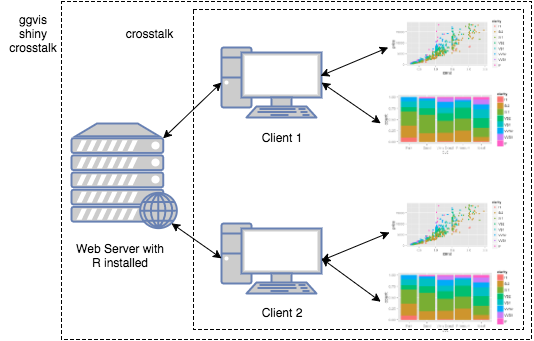
\includegraphics{diagrams/server-client} 

}

\caption{A basic visual depiction of the different approaches to implementing a data pipeline for interactive web graphics. The R packages **ggvis** and **shiny** expose the pipeline to users in R, which requires a web server for viewing. The R package **crosstalk** will allow developers to implement and expose the pipeline on both the server and client levels.}\label{fig:server-client}
\end{figure}

Generally speaking, websites that render entirely client-side are more
desirable since they are easier to share, more responsive, and require
less computational resources to run\footnote{The
  \url{http://www.shinyapps.io/} service helps to provide easy access to
  a \textbf{shiny} server (a web server running special shiny software),
  so that \textbf{shiny} apps can be shared via a URL, for example:
  \url{https://hadley.shinyapps.io/14-ggvis/linked-brushing.Rmd}}.
However, the client-server approach can be very useful for dynamically
performing statistical computations, a key characteristic of most
interactive statistical graphics systems. \citep{FastRWeb} and
\citep{opencpu} also allow us to execute R code on a web server, and
retrieve output via HTTP, but \textbf{shiny} is the most heavily used
since apps can be written entirely in R using a very powerful, yet
approachable, reactive programming framework for handling user events.
There are also many convenient shortcuts for creating attractive HTML
input forms, making it incredibly easy to go from R script to an web app
powered by R that dynamically updates when users alter input values. In
other words, \textbf{shiny} makes it quick and easy to write web-based
GUIs with support for indirect manipulation.

Historically, an advanced understanding of \textbf{shiny} and JavaScript
was required to implement direct manipulation in a \textbf{shiny} app.
Recently, \textbf{shiny} added support for retrieving information on
user events with static R graphics\footnote{This website shows what
  information is sent from the client to the server when users interact
  with plot(s) via mouse event(s) --
  \url{http://shiny.rstudio.com/gallery/plot-interaction-basic.html}},
allowing developers to coordinate views in a web app, with no JavaScript
involved. This is a powerful tool for R users, but it has its
weaknesses. Most importantly, its not clear how to handle interactions
when positional scales are categorical (e.g., a bar chart) or how to
provide a visual clue that something has been selected.

The touring video in Figure \ref{fig:tour} purposefully uses
\textbf{shiny}'s built-in support for brushing to demonstrate the
problem with providing a visual clue. This points to the fundamental
problem in using non-web-based graphics to implement interactive
graphics in a web browser: every time the view updates, the display must
be redrawn, resulting in a ``glitch'' effect. If the plot being brushed
used native web graphics (e.g., SVG), it would allow for finer control
over how the view updates in response to user interactions and/or
dynamic data. On the other hand, since \textbf{ggvis} is web-based, and
has special client-side functionality, it knows how to smoothly
transition from one frame to the next when provided with new data from
the \textbf{shiny} server, which is crucial for constructing a mental
model of the data space. Having richer interfaces for generating
web-based interactive graphics from R that can share selections, and
handle smooth transitions, would make this, and many other examples,
generally better.

Many web-based graphing toolkits have appeared since the advent of
\textbf{rCharts}, making a single package that interfaces with
\emph{every} toolkit infeasible. Some ideas deriving from work on
\textbf{rCharts}, such as providing the glue to render plots in various
contexts (e.g., the R console, shiny apps, and \textbf{rmarkdown}
documents), have evolved into the R package \textbf{htmlwidgets}
\citep{htmlwidgets}. Having built similar bridges for \textbf{animint}
and \textbf{LDAvis}, I personally know and appreciate the amount of time
and effort this package saves other package authors.

The \textbf{htmlwidgets} framework is not constrained to just graphics,
it simply provides a set of conventions for authoring web content from
R. Numerous JavaScript data visualization libraries are now made
available using this framework, most designed for particular use cases,
such as \textbf{leaflet} for geo-spatial mapping, \textbf{dygraphs} for
time-series, and \textbf{networkD3} for networks \citep{leaflet};
\citep{dygraphs}; \citep{networkD3}.\footnote{For more examples and
  information, see \url{http://www.htmlwidgets.org/} and
  \url{http://hafen.github.io/htmlwidgetsgallery/}} There are also HTML
widgets that provide an interface to more general purpose visualization
JavaScript libraries such as \textbf{plotly}, \textbf{rbokeh}, and
\textbf{rcdimple} \citep{plotly}; \citep{rbokeh}; \citep{rcdimple}. Most
of these JavaScript libraries provide at least some native support for
direct manipulation such as identifying (i.e., mousing over points to
reveal labels), focusing (i.e., pan and zoom), and sometimes
highlighting (i.e., brushing over points to highlight points in another
view). More often than not, the support for dynamic and linked views is
lacking, especially if we want to define the linking in R, and produce a
standalone HTML document.

The R package \textbf{crosstalk} is a new framework for coordinating
arbitrary HTML widgets \citep{crosstalk}. It provides both an R and a
JavaScript API for querying selections, meaning \textbf{crosstalk}
powered HTML widgets can work with or without \textbf{shiny}, and if
implemented carefully by HTML widget authors, provides a means for
coordinating multiple HTML widgets without shiny. Generally speaking,
\textbf{crosstalk} just provides a standard way to set, store, and
access selection values in the browser, so the actual logic for updating
views based on the selection value(s) is on the HTML widget author, and
this part is far from trivial. In a sense, this project is similar to
the work of \citet{North:1999vi}, which provides semantics for
``snapping together'' arbitrary views that are aware of the relational
schema, but does so in a web-based environment, rather than requiring a
machine running Windows.

The first HTML widget to leverage \textbf{crosstalk} was
\citep{d3scatter}, but is limited to linked brushing on
scatterplots.\footnote{See, for example,
  \url{http://rpubs.com/jcheng/crosstalk-demo}} Currently, there are a
couple other R packages with \textbf{crosstalk} support, including
\textbf{leaflet} and \textbf{listviewer}, but \textbf{plotly} is the
only package which supports a non-identity functions between the data
and displays. It also has rich support for interaction types, including
mouse hover, click, and multiple types of click+drag selections.

Having HTML widgets that can share selections with each other will be a
huge step forward for web-based interactive graphics. With some effort
and careful implementation by HTML widget authors, it may be possible to
provide sensible defaults for updating views between arbitrary widgets,
and users that know some JavaScript will also be able to customize or
extend these defaults from R. The \textbf{htmlwidget} package provides
conventions for this, by allowing one to send arbitrary JavaScript
functions from R that execute after the widget has rendered in the
browser. The biggest problem in implementing coordinated widgets will be
in managing data structures, since each widget will likely have its own
data structure for representing a selection. In this case, in order to
coordinate them, users may have to embed widgets in a shiny app to
access and organize selections. This gives users tremendous control over
sharing selections, but may limit control over smooth transitions
between states of a given widget (a key characteristic of dynamic
graphics), and increases the amount of complexity involved in sharing
their work.

\hypertarget{taming-pitchfx-data-with-xml2r-and-pitchrx}{\chapter{Taming
PITCHf/x Data with XML2R and
pitchRx}\label{taming-pitchfx-data-with-xml2r-and-pitchrx}}

Pitch f/x refers a massive, publicly available baseball dataset hosted
on the web in XML and JSON format. Since this data is large, increases
on a daily basis, and only licensed for individual use, the
\textbf{pitchRx} package provides a simple interface to download, parse,
clean, and transform the data from its source (instead of directly
distributing the data). If acquiring large amounts of data, to avoid
memory limitations, users may divert incoming data in chunks to a
database using any valid R database connection \citep{DBI}. It also
provides a convenient function to update an existing database with the
most recently available data without re-downloading anything.

The \textbf{openWAR} package also provides high-level access to Pitch
f/x data, but it is currently more limited in the data it can acquire
\citep{openWAR}. It also currently depends on the difficult to install
\textbf{Sxslt} package, impeding portability \citep{Sxslt}.
\textbf{openWAR} depends on \textbf{Sxslt} to help transform XML files
to R data frames via XSL Transformations (XSLT). Without advanced
knowledge of XSLT, one must define transformations by hard coding
assumptions about the XML format, such as the names of fields of
interest. New variables have been added into Pitch f/x several times,
and \textbf{pitchRx} automatically picks them up, thanks to
functionality provided by \textbf{XML2R}.

\textbf{XML2R} makes it easy to wrangle relational data stored as a
collection of XML files into a list of data frames. Its interface
satisfies principles from pure functional programming: the output of
each function can be completely determined from the input. The interface
is also predictable: each function inputs and outputs a list of
observations (an observation is a matrix with one row). It also
represents XML content as a list of observations (matrices with one
row), allowing each function to operate on native R data structures,
making it more intuitive for R programmers to work with compared to the
non-native XMLDocumentContent. This new representation is slightly less
computationally efficient in some cases, but it has also made it much
easier to implement and maintain higher-level interfaces to specific XML
data sources, such as \textbf{pitchRx} and \textbf{bbscrapeR}
\citep{bbscrapeR}.

To see the fully published article ``Taming PITCHf/x Data with XML2R and
pitchRx'', see
\url{http://rjournal.github.io/archive/2014-1/sievert.pdf}

\hypertarget{ldavis-a-method-for-visualizing-and-interpreting-topics}{\chapter{LDAvis:
A method for visualizing and interpreting
topics}\label{ldavis-a-method-for-visualizing-and-interpreting-topics}}

The R package \textbf{LDAvis} creates an interactive web-based
visualization of a topic model that has been fit to a corpus of text
data using Latent Dirichlet Allocation (LDA). Given the estimated
parameters of the topic model, it computes various summary statistics as
input to a reusable interactive visualization built with HTML,
JavaScript, and D3. The goal is to help users interpret the topics in
their LDA topic model, and the interactive visualization is primarily
useful for quickly viewing, altering, and tracking changes in rankings
of terms for a given topic.

In a topic model, each topic is defined by a probability mass function
over each unique term in the corpus. When studying their differences,
analysts often look at lists of the top (say 30) terms of a topic ranked
by the estimated probability within that given topic. As discussed in
the video below and in our paper, this makes it hard to differentiate
meaning between topics since words that are likely to appear overall are
also likely to appear in a given topic. Instead, we propose ranking
terms using a compromise between this probability and lift (probability
within topic divided by overall probability). We also conduct a user
study which provides evidence that this compromise helps in identifying
topics, and propose a sensible starting point for choosing a compromise;
but in practice, users will want to adjust this value and understand how
rankings are affected. For this reason, it is important that we assist
users in their ability to track changes, by using smooth transitions
from one ranking to the next.

To read the full paper, see:
\url{http://nlp.stanford.edu/events/illvi2014/papers/sievert-illvi2014.pdf}

\chapter{Two new keywords for interactive, animated plot design:
clickSelects and
showSelected}\label{two-new-keywords-for-interactive-animated-plot-design-clickselects-and-showselected}

This paper explains the clickSelects/showSelected paradigm, implemented
in \textbf{animint}, which makes it easy to select/query points
belonging to arbitrary group(s) and visualize those points in another
data space. This differs from the classical linked brushing approach
where points must belong to contiguous regions within a subset of the
data space.

\url{https://github.com/tdhock/animint-paper/blob/master/HOCKING-animint.pdf}

\chapter{Interactive Data Visualization with plotly and
shiny}\label{interactive-data-visualization-with-plotly-and-shiny}

\citet{Cook:2007uk} proposed a taxonomony of interactive data
visualization based on three fundamental data analysis tasks: finding
Gestalt, posing queries, and making comparisons. The top-level of the
taxonomy comes in two parts: \emph{rendering}, or what to show on a
plot; and \emph{manipulation}, or what to do with plots.{[}\^{}The
cookbook and advanced manipulation sections of the plotly book{]} Under
the manipulation branch, they propose three branches of manipulation:
focusing individual views (for finding Gestalt), linking multiple views
(for posing queries), and arranging many views (for making comparisons).
Of course, each of the three manipulation branches include a set of
techniques for accomplishing a certain task (e.g., within focusing
views: controlling aspect ratio, zoom, pan, etc), and they provide a
series of examples demonstrating techniques using the XGobi software
toolkit \citep{xgobi}.

This paper explores the taxonomy proposed by \citet{Cook:2007uk} in
detail, and demonstrates how we can bring these techniques to the web
browser via the R packages \textbf{plotly} and \textbf{shiny}
\citep{plotly}; \citep{shiny}.

\section{The taxonomy}\label{the-taxonomy}

\section{Exploring Australian election
data}\label{exploring-australian-election-data}

\section{Exploring pedestrain counts}\label{exploring-pedestrain-counts}

\section{Exploring disease outbreaks}\label{exploring-disease-outbreaks}

\begin{itemize}
\tightlist
\item
  Geographic zoom+pan linked to summary statistics. Fosters all three
  tasks?
\item
  Explain how
\end{itemize}

\chapter{References}\label{references}

\hypertarget{refs}{}

% might need this -- https://github.com/robjhyndman/monashthesis/blob/master/monashthesis.tex
%\printbibliography

\end{document}
